\documentclass[12pt,oneside]{uhthesis}
\usepackage{subfigure}
\usepackage[ruled,lined,linesnumbered,titlenumbered,algochapter,spanish,onelanguage]{algorithm2e}
\usepackage{amsmath}
\usepackage{amssymb}
\usepackage{amsbsy}
\usepackage{caption,booktabs}
\captionsetup{ justification = centering }
%\usepackage{mathpazo}
\usepackage{float}
\setlength{\marginparwidth}{2cm}
\usepackage{todonotes}
\usepackage{listings}
\usepackage{xcolor}
\usepackage{multicol}
\usepackage{graphicx}
\floatstyle{plaintop}
\restylefloat{table}
\addbibresource{Bibliography.bib}
% \setlength{\parskip}{\baselineskip}%
\renewcommand{\tablename}{Tabla}
\renewcommand{\listalgorithmcfname}{Índice de Algoritmos}
%\dontprintsemicolon
\SetAlgoNoEnd

\definecolor{codegreen}{rgb}{0,0.6,0}
\definecolor{codegray}{rgb}{0.5,0.5,0.5}
\definecolor{codepurple}{rgb}{0.58,0,0.82}
\definecolor{backcolour}{rgb}{0.95,0.95,0.92}

\lstdefinestyle{mystyle}{
    backgroundcolor=\color{backcolour},   
    commentstyle=\color{codegreen},
    keywordstyle=\color{purple},
    numberstyle=\tiny\color{codegray},
    stringstyle=\color{codepurple},
    basicstyle=\ttfamily\footnotesize,
    breakatwhitespace=false,         
    breaklines=true,                 
    captionpos=b,                    
    keepspaces=true,                 
    numbers=left,                    
    numbersep=5pt,                  
    showspaces=false,                
    showstringspaces=false,
    showtabs=false,                  
    tabsize=4
}

\lstset{style=mystyle}

\title{Transistor, microchip y microprocesador}
\author{\\\vspace{0.25cm}Javier E. Domínguez Hernández. C-412\\\vspace{0.2cm} David Orlando De Quesada Oliva. C-411}
% \advisor{\\\vspace{0.25cm}Yudivián Almeida\\\vspace{0.2cm}Carlos Bermudez Porto}
% \degree{Licenciado en (Matemática o Ciencia de la Computación)}
\faculty{Facultad de Matemática y Computación}
\date{Fecha\\\vspace{0.25cm}20 de octubre de 2022}
\logo{Graphics/uhlogo}
\makenomenclature

\renewcommand{\vec}[1]{\boldsymbol{#1}}
\newcommand{\diff}[1]{\ensuremath{\mathrm{d}#1}}
\newcommand{\me}[1]{\mathrm{e}^{#1}}
\newcommand{\pf}{\mathfrak{p}}
\newcommand{\qf}{\mathfrak{q}}
%\newcommand{\kf}{\mathfrak{k}}
\newcommand{\kt}{\mathtt{k}}
\newcommand{\mf}{\mathfrak{m}}
\newcommand{\hf}{\mathfrak{h}}
\newcommand{\fac}{\mathrm{fac}}
\newcommand{\maxx}[1]{\max\left\{ #1 \right\} }
\newcommand{\minn}[1]{\min\left\{ #1 \right\} }
\newcommand{\lldpcf}{1.25}
\newcommand{\nnorm}[1]{\left\lvert #1 \right\rvert }
\renewcommand{\lstlistingname}{Ejemplo de código}
\renewcommand{\lstlistlistingname}{Ejemplos de código}

\begin{document}

\frontmatter
\maketitle

% \include{FrontMatter/Dedication}
% \include{FrontMatter/Thanks}
% \include{FrontMatter/SupervisorOpinion}
\begin{resumen}
	Una síntesis de que personalidades participaron a lo largo de la historia en la
	creación del transistor, el microchip y el microprocesador, y como fue el camino
	para la invención de estos importantes componentes que forman parte no solo de la
	computadora actual, sino también de la gran mayoría de los dispositivos electrónicos
	que usamos en el día a día. 
\end{resumen}

\begin{abstract}
	A synthesis of which personalities participated throughout history in the
	creation of the transistor, the microchip and the microprocessor, and how was the path
	for the invention of these important components that are part not only of the
	current computer, but also the vast majority of electronic devices
	that we use on a daily basis.
\end{abstract}

\textbf{Keywords}: transistor, microchip, microprocesador, computación, descubrimiento, hardware
\tableofcontents
\listoffigures
% \listoftables
% \listofalgorithms
% \lstlistoflistings

\mainmatter

% \include{MainMatter/Introduction}
\chapter{El transistor}\label{chapter:transistor}

Antes de la invención del primer transistor a finales de la década de 1930, ya existían dispositivos que cumplían la misma función que 
este pero con una menor eficiencia.\\
\indent A finales del siglo XIX con el incipiente desarrollo de la tecnología de comunicación inalámbrica y la construcción de sistemas
que utilizaran este método por la \emph{compañía Marconi}, \emph{Guglielmo Marconi} le asignó el cargo de consejero científico al físico
inglés \emph{John Ambrose Fleming}. \emph{Marconi} necesitaba ayuda para mejorar el \textbf{detector}, que es el dispositivo que se
encarga de extraer información de una corriente de radiofrecuencia modulada, y aunque ya él había desarrollado un \textbf{detector
magnético}, este solo brindaba una señal de frecuencia de audio a un receptor de teléfono. Un \textbf{detector} confiable que pudiera
guiar un instrumento de impresión era necesario. Fleming pudo desarrollar un \textbf{tubo al vacío} como resultado de su trabajo con
\textbf{bombillas de efecto Edison}, a estas las denominó \textbf{válvulas de oscilación} ya que pasaba corriente en una sola dirección.
Fleming presentó una patente para estos tubos, cedida a la \emph{compañía Marconi} en el Reino Unido en noviembre de 1904 y esta se emitió
en septiembre de 1905. Conocida más tarde como la \textbf{válvula Fleming}, la \textbf{válvula de oscilación} se desarrolló con el fin de
rectificar la corriente de radiofrecuencia como componente detector de circuitos receptores de radio. \brackcite{wikipedia_2022_tube}\\
\indent En el propio siglo XIX ingenieros de telégrafos y teléfono habían reconocido la necesidad de incrementar la distancia que la señal
pudiera ser transmitida. En 1906 \emph{Robert Von Lieben} solicitó una patente para un \textbf{tubo de rayos catódicos} que usaba una bobina
de deflexión magnética externa y estaba destinado a usarse como amplificador en equipos de telefonía. A \emph{Lee de Forest} se le acredita
la invención del tubo triodo en 1907, el cual tenía la capacidad de amplificar las señales, y que fue el primero de su tipo que tuvo uso
práctico. Sin embargo estos \textbf{tubos de vacío} utilizados para amplificar la música y la voz que hicieron posibles las llamadas de
larga distancia, creaban mucho calor y se quemaban muy rápido, requiriendo alto mantenimiento. \brackcite{wikipedia_2022_tube, wikipedia_2022_triode}\\
\indent La \textbf{ENIAC}(\emph{Electronic Numerical Integrator and Computer}) fue la primera computadora en usar los \textbf{tubos de vacío},
exactamente 18 000 de estos para poder funcionar, que hicieron que aquel dispositivo ocupara el tamaño de una habitación completa. Estos tubos
permitían que las señales fueran enviadas y los cálculos realizados de forma más rápida a través del uso de conmutación eléctrica en vez de
conmutación mecánica. Debido al enorme consumo de energía eléctrica de la \textbf{ENIAC}, muchas personas creyeron que esta se destruiría,
sin embargo los \textbf {tubos de vacío} le permitieron soportar y funcionar. ~\brackcite{richards_2022}.\\

\begin{figure}[htb]
	\centering
	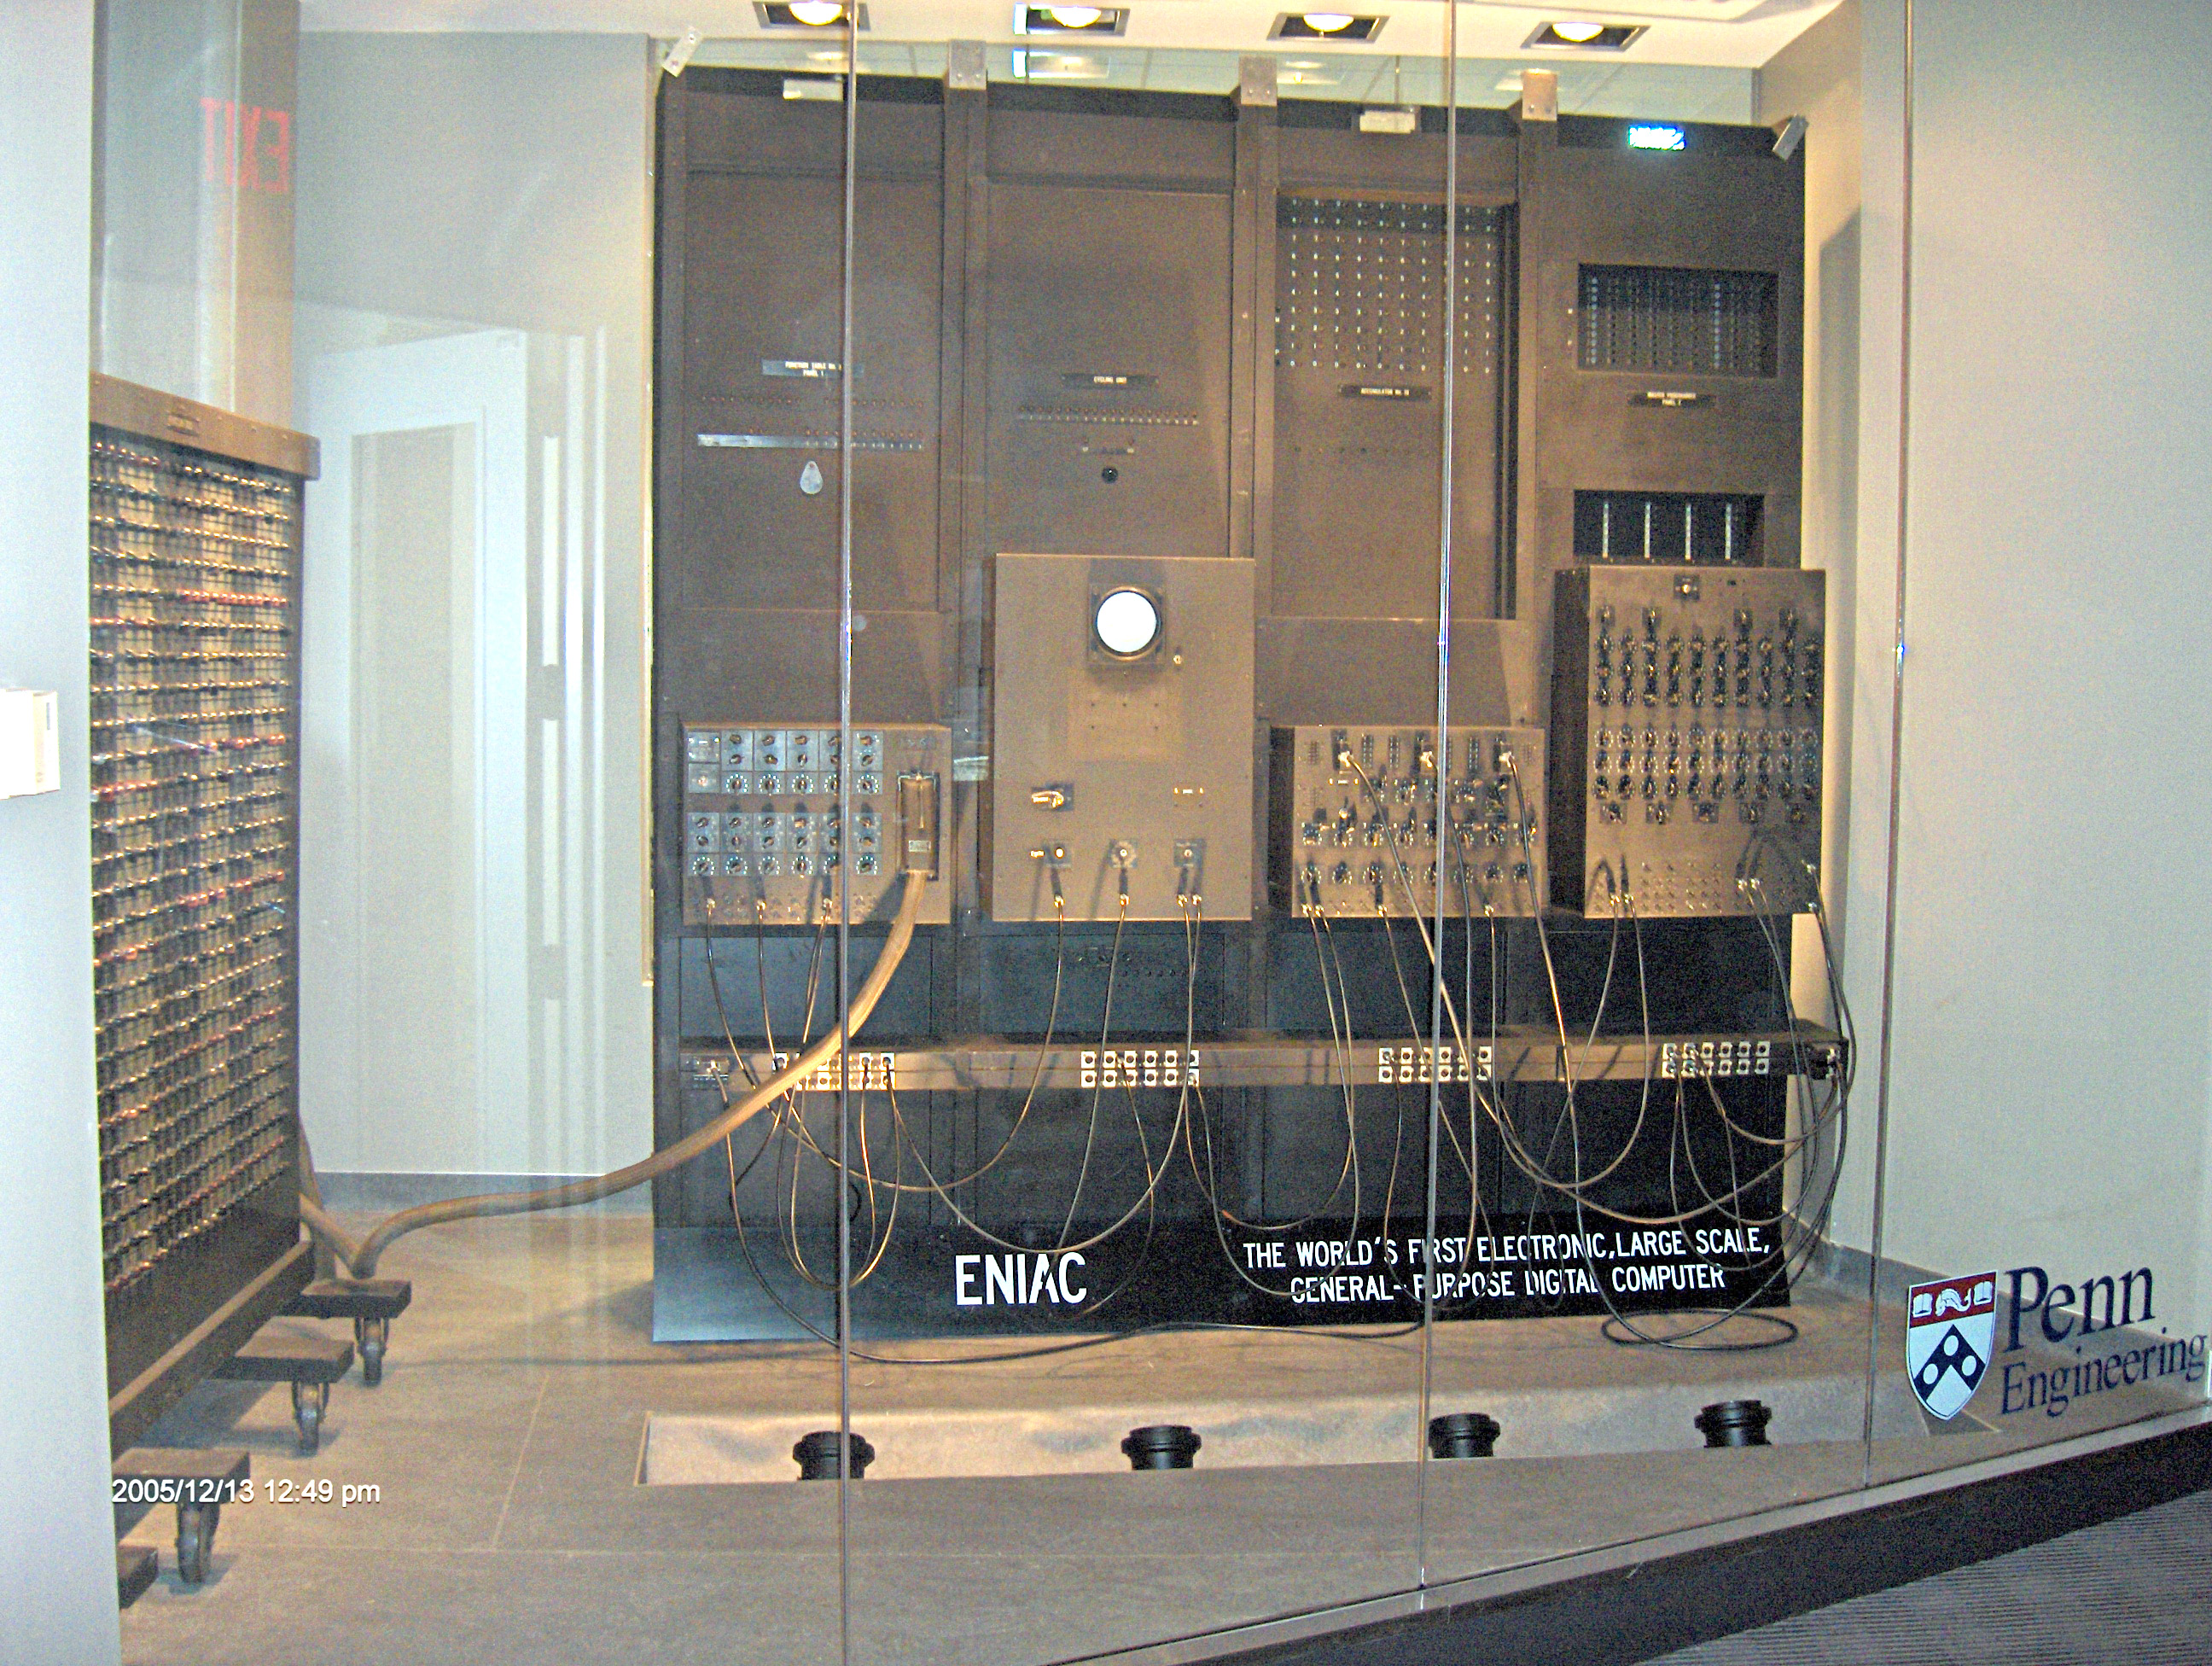
\includegraphics[scale = 0.13]{Graphics/ENIAC.jpg}
	\caption{\textbf{ENIAC} primera computadora que utilizó los \textbf{tubos de vacío}.}
	\label{fig:1}
\end{figure}

\section{El surgimiento}
Debido a que las computadoras dependían de los \textbf{tubos de vacío} tan frágiles, grandes,
costosos y con un consumo enorme de energía, solo las grandes compañías, los militares y las
universidades con proyectos de investigación podían permitírselas. Por esta razón el inicio de la
era digital, aquella donde los dispositivos electrónicos se convertirían en una parte indispensable
en nuestro día a día, no ocurriría sino hasta el martes 16 de diciembre de 1947. Ese día 2 científicos
en los \emph{laboratorios Bell} lograron armar un pequeño artilugio que habían inventado a partir de
unas tiras de oro, papel de aluminio, un trozo de material semiconductor(\textbf{germanio}) y un sujetapapeles
doblado, el cual movido a la perfección podía amplificar una corriente eléctrica y encenderla y apagarla.\\
Durante mucho tiempo hubo una persona encargada de encontrar un reemplazo para los \textbf{tubos 
de vacío}, un reemplazo menos costoso, más sólido y más barato, esa persona fue el físico experto
en estado sólido \emph{William Shockley}, graduado del \textbf{MIT}(\emph{Massachussets Institute of Technology}),
quien fue contratado por \emph{Mervin Kelly} jefe del departamente de \textbf{tubos al vacío} de los \emph{
labotorios Bell} con este fin. Luego de 3 años a \emph{Shockley} se le ocurrió que podría encontrar una
solución utilizando materiales sólidos como el \textbf{silicio} en vez de los filamentos de una bombilla, “Se 
me ha ocurrido que es posible crear un amplificador utilizando semiconductores en vez del vacío",
escribió \emph{Shockley}. Él parecía tener la capacidad de visualizar la teoría cuántica por cómo explicaba
el movimiento de los electrones. Sus colegas decían que podía mirar material semiconductor y ver los
electrones. Sin embargo, para transformar su intuición en un invento real, \emph{Shockley} necesitaba
un socio que fuera un hábil experimentador, y fue \emph{Walter Brattain} quien disfrutaba creando
dispositivos con semiconductores quien se unió a \emph{Shockley} en su tarea. Lamentablemente sus
ideas tuvieron que esperar pues recién comenzó la II Guerra Mundial, y no fue hasta casi 4 años
después que regresaron a su trabajo en los laboratorios que retomaron su investigación, y fueron
asignados a un grupo cuyo objetivo principal era encontrar el tan buscado reemplazo sólido para
los \textbf{tubos de vacío} utilizando semiconductores. Esta vez decidieron incorporar al grupo un 
nuevo teórico además de \emph{Shockley}, experto en teoría cuántica, \emph{John Bardeen}, un niño
genio que se había saltado tres grados en la escuela, \emph{Bardeen } había trabajado durante su servicio
en tiempos de guerra en la Artillería Naval y discutió el diseño de torpedos con nada más ni nada menos que 
\emph{Albert Einstein}. Él era uno de los mejores expertos del mundo en el uso de la teoría cuántica
para comprender cómo materiales conducen la electricidad, y tenía, según sus colegas, una “capacidad genuina
para colaborar fácilmente con experimentadores y teóricos". Así, ya se habían juntados los 3 hombres más importantes
de este proyecto. \brackcite{isaacson_2014}\\
\newpage

\begin{figure}[htb]
	\centering
	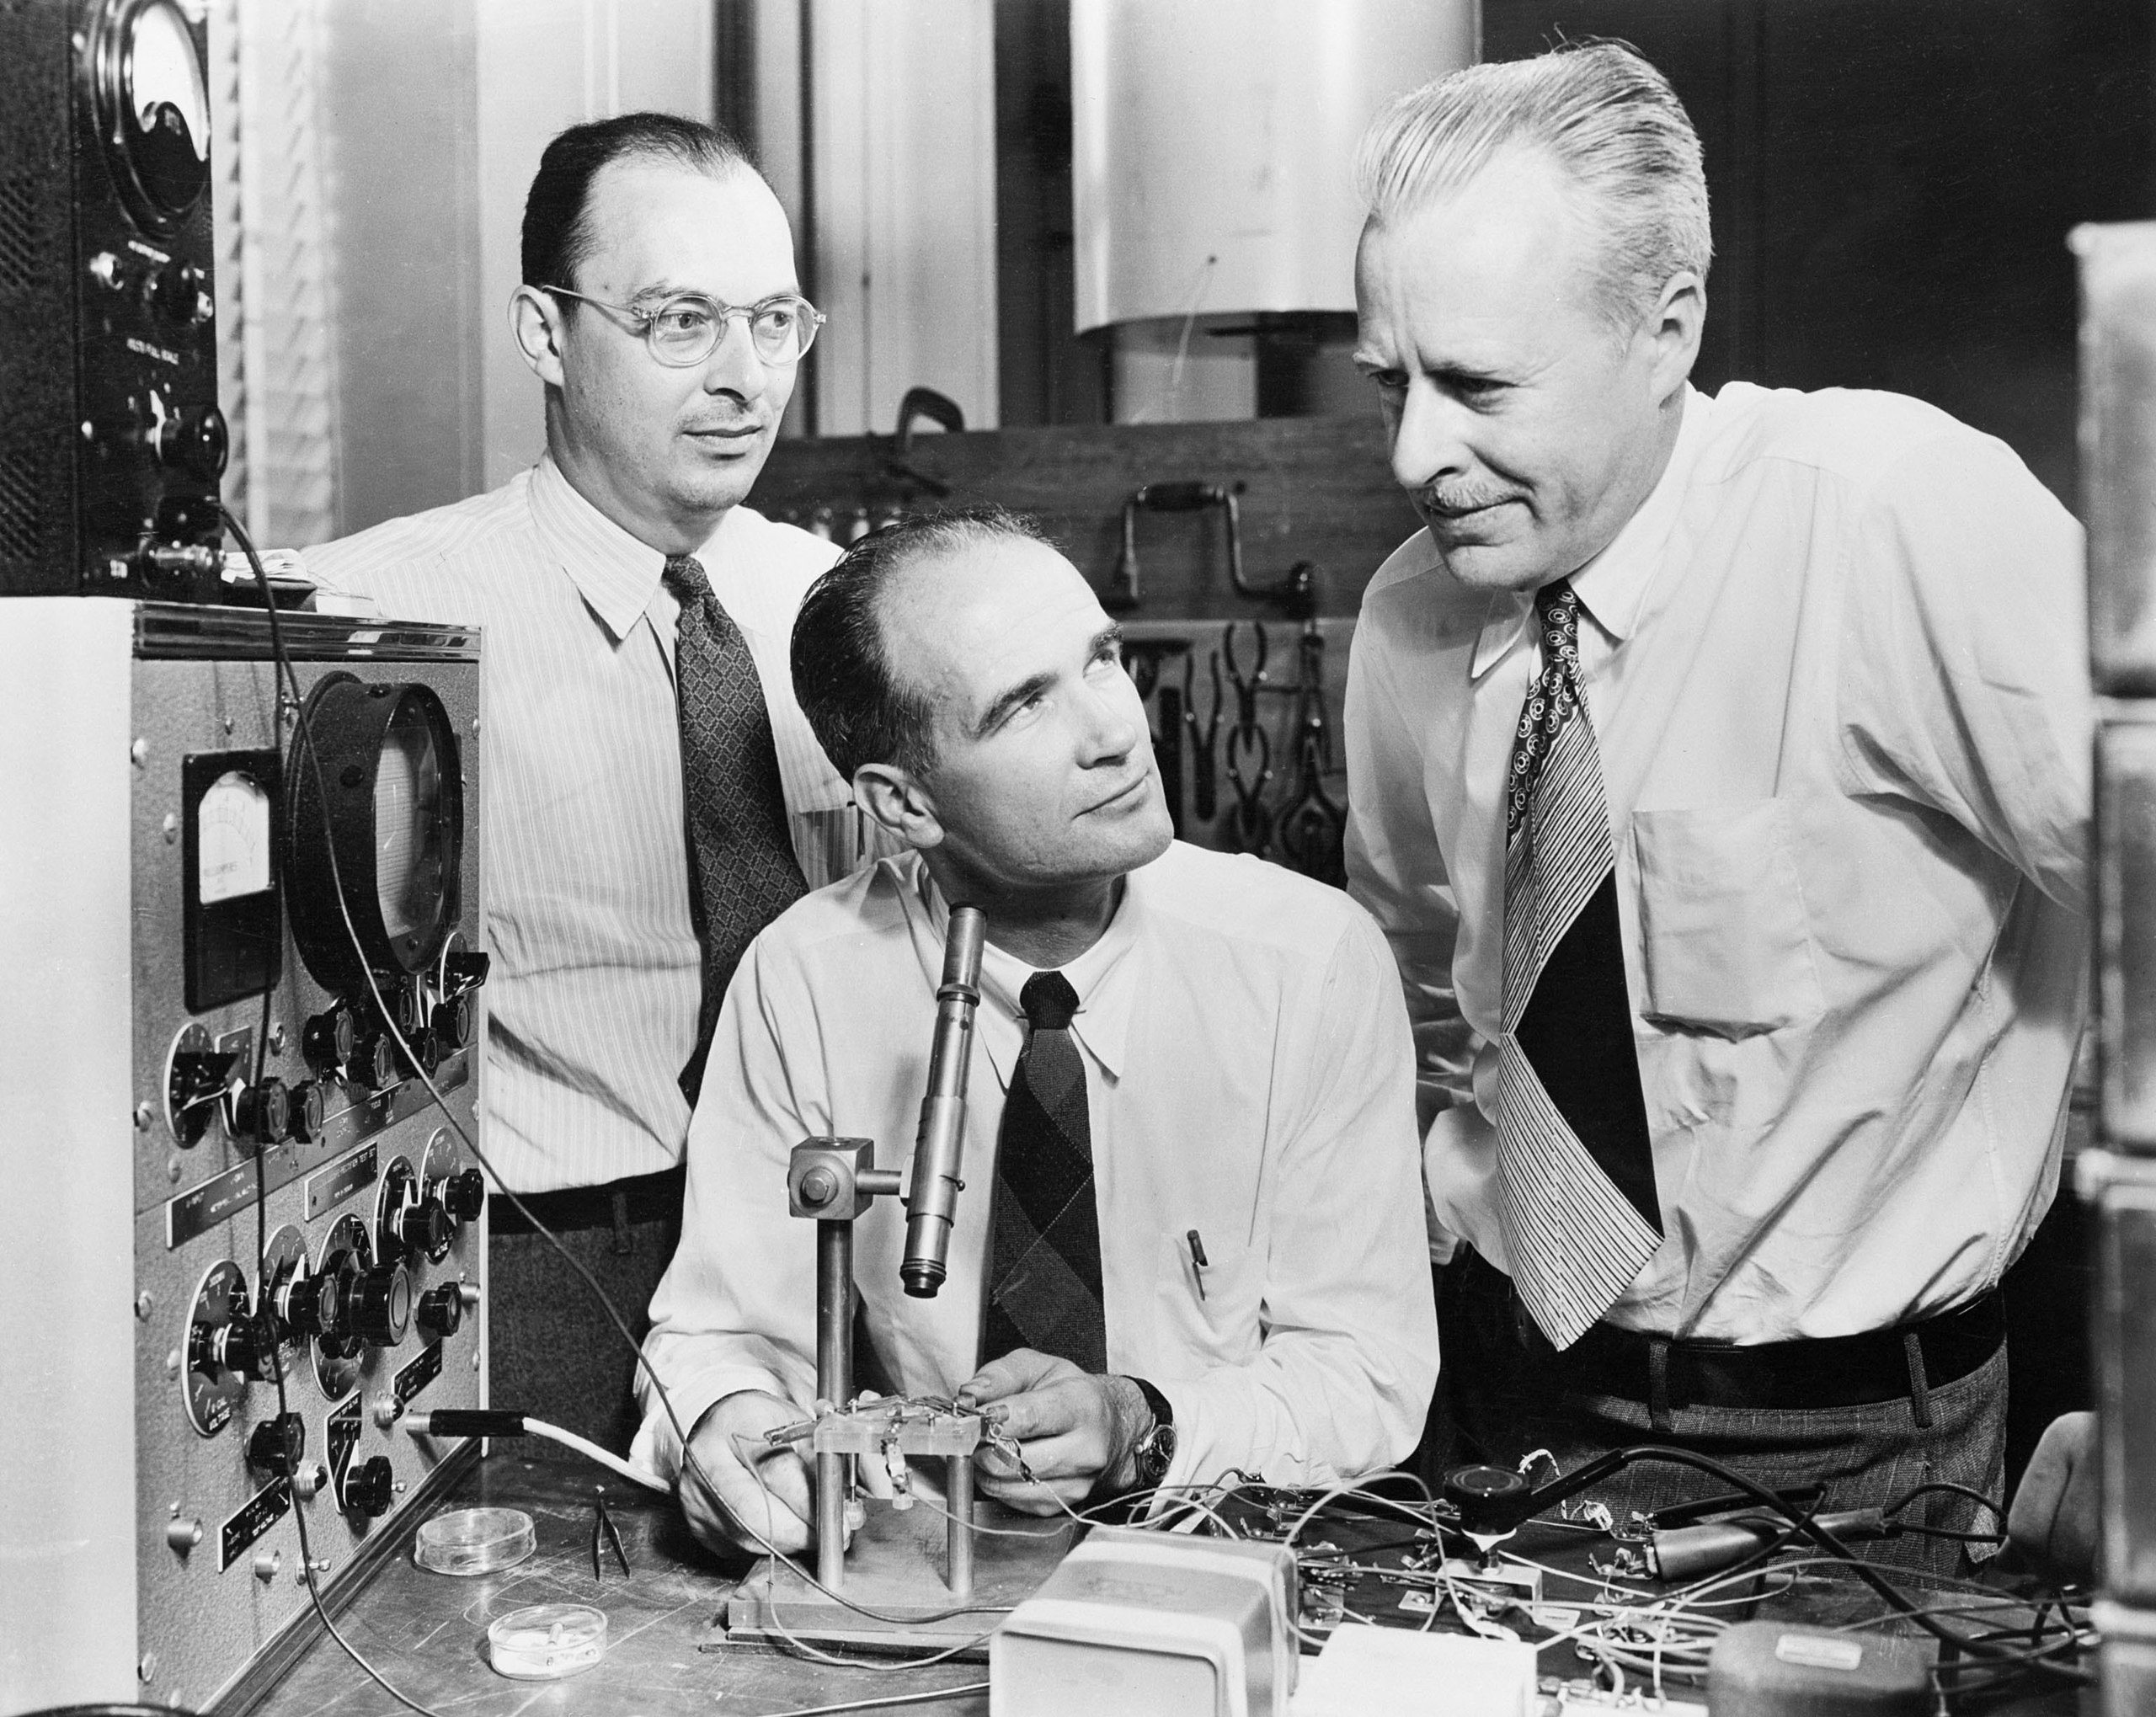
\includegraphics[scale = 0.13]{Graphics/Bardeen_Shockley_Brattain_1948.jpg}
\caption{\emph{John Bardeen, William Shockley} y \emph{Walter Brattain}, de izquierda a derecha en 1948.}
	\label{fig:2}
\end{figure}

Las más sorprendentes ideas provinieron de las interacciones entre ellos. "La cercana y constante colaboración entre
experimentalistas y teóricos se extendió a través de todas las etapas de la investigación, desde la concepción del
experimento hasta los análisis de los resultados”, dijo \emph{Bardeen}. Gracias a esta estrecha colaboración fue que 
el 16 de diciembre de 1947 lograron crear el primer \textbf{transistor} de la historia.\\

\begin{figure}[htb]
	\centering
	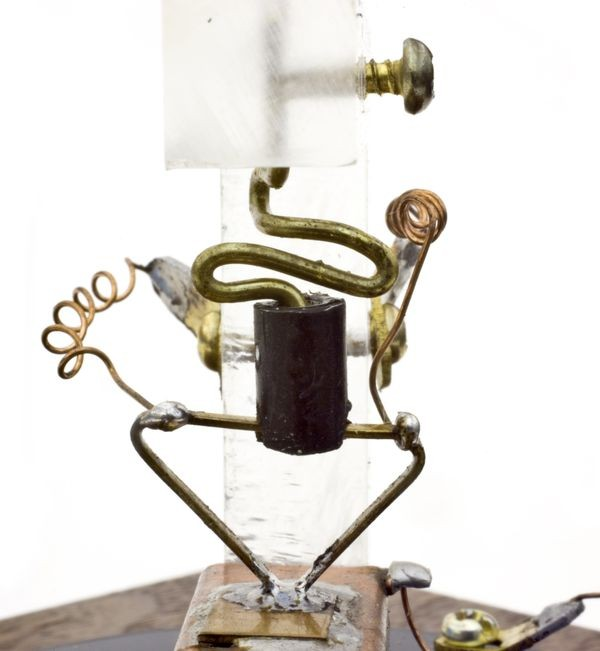
\includegraphics[scale = 0.2]{Graphics/first_transistor_replica.jpg}
	\caption{Réplica del primer \textbf{transistor}.}
	\label{fig:3}
\end{figure}

Los \emph{laboratorios Bell} fueron el fruto de un inmenso trabajo y hasta cierto punto una apuesta de la \textbf{AT\&T}
(\emph{American Telephone and Telegraph Company}) que a principios de 1907 pasaba por una grave crisis, y con la guía
\emph{Alexander Graham Bell}, \emph{Theodore Vail} y el apoyo de la junta directiva lograron salvar a la empresa de la quiebra,
y a la vez juntar un gran talento en este lugar, teóricos, científicos de materiales, metalúrgicos, ingenieros e incluso escaladores
de postes de \textbf{AT\&T}, y fueron 3 de estos talentosos expertos los que hicieron el descubrimiento, sin embargo la invención del
\textbf{transistor} no fue el resultado del trabajo de solo ellos 3, fue la mezcla del conocimiento de diversos talentos presentes
desde el inicio en los \emph{laboratorios Bell}, e incluso antes. Como escribiera \emph{William Shockley} “Son necesarios muchos hombres
de varios campos de la ciencia, juntando su talento, para poder llevar a cabo toda la investigación necesaria para el desarrollo de un
nuevo dispositivo". Tiempo después, los 3 descubridores serían galardonados con el \emph{Premio Nobel} en física por sus investigaciones con 
semiconductores y su descubrimiento sobre el \textbf{transistor}. \brackcite{wikipedia_2022_history_transistor, isaacson_2014}\\

\section{Primeras aplicaciones}
La primera línea de producción comercial de transistores del mundo se encontraba en la planta de \emph{Western Electric} en \emph{Union Boulevard}
en \emph{Allentown}, \emph{Pensilvania}. La producción comenzó el 1 de octubre de 1951 con el \textbf{transistor de germanio de contacto puntual}.
La primera aplicación comercial de transistores en telecomunicaciones fue en el otoño de 1952 en generadores de tonos para señalización multifrecuencia
del sistema de conmutación de barra transversal No. 5 en la instalación de \emph{Englewood}, \emph{Nueva Jersey}, utilizada para la primera prueba de
campo de marcación directa a distancia (DDD). Para 1953, el transistor se usaba en algunos productos, como audífonos y centrales telefónicas, pero aún
había problemas importantes que impedían su aplicación más amplia, como la sensibilidad a la humedad y la fragilidad de los cables conectados a los
cristales de \textbf{germanio}.\brackcite{wikipedia_2022_history_transistor}\\ 
En la primavera de 1952, \emph{Pat Haggerty} el presidente de la companía \emph{Texas Instruments}, que recién había dejado el campo de la exploración
de petróleo por los transistores pues su presidente estaba convencido de que cambiaría el mundo por completo, y creían que lograrían aprovechar
este recién descubierto artilugio para su beneficio. El problema era que las personas en los \emph{Laboratorios Bell} eran escéptios de si serían capaces
de lograrlo, por lo que se negaban a darles una licencia para hacer uso de la nueva tecnología, al menos en un principio. Sin embargo, en la primavera de
1952 \emph{Haggerty} logró covencerlos de que les vendieran una licenia para fabricar el \textbf{transistor}. Él también contrató a \emph{Gordon Teal},
un investigador químico que trabajó en uno de los largos pasillos de los \emph{Laboratorios Bell} cerca del equipo de semiconductores. \emph{Teal} era
un experto en la manipulación de \textbf{germanio}, pero cuando se unió a \emph{Texas Instruments} había cambiado su interés al \textbf{silicio}, un
elemento más abundante que podía funcionar mejor a altas temperaturas. De esta forma en mayo de 1954, pudo fabricar un transistor de \textbf{silicio} que usaba la
\textbf{unión n-p-n} arquitectura desarrollada por \emph{Shockley}, lo que permitió, más adelante, reducir el precio de los transistores de \$16 a solo \$3,
facilitando que el \textbf{transistor} pudiera llegar al mercado consumidor. Para junio de 1954 \emph{Haggerty} había llegado a un acuerdo con una pequeña 
companía de \emph{Indianapolis} que fabriaba amplificadores para antenas, para juntos crear lo que llamarían el radio \textbf{Regency TR-1}, que salió a la venta 
por \$49.95. \brackcite{isaacson_2014}\\

\begin{figure}[htb]
	\centering
	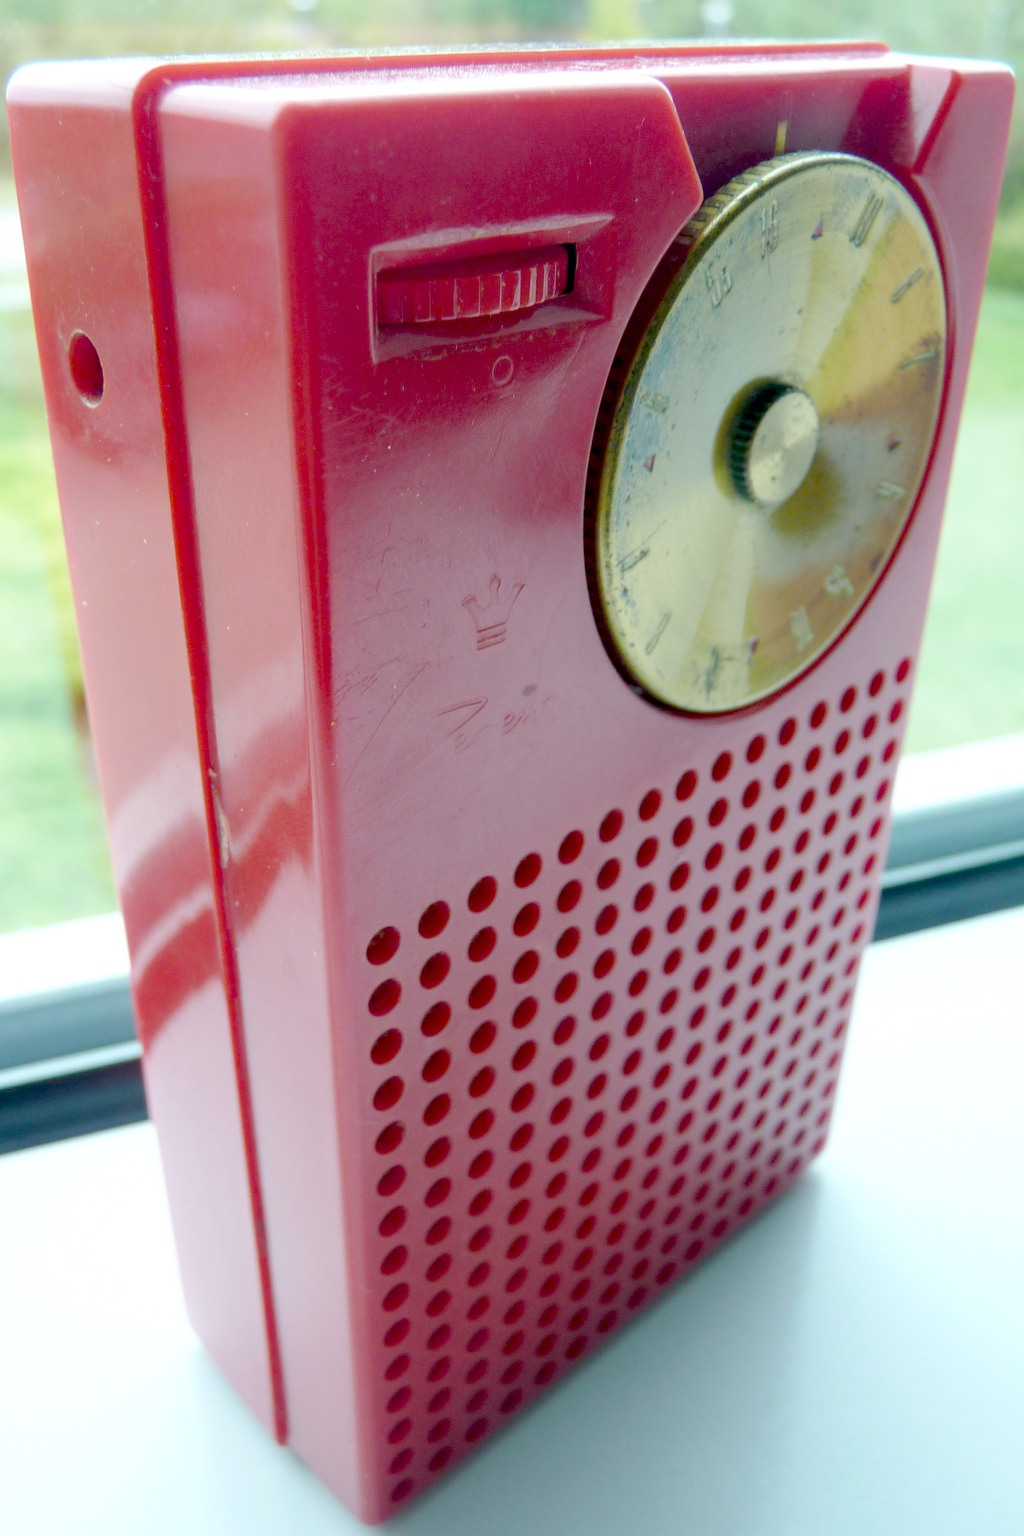
\includegraphics[scale = 0.2]{Graphics/Regency_TR-1_radio.jpg}
	\caption{Radio \emph{Regency TR-1}.}
	\label{fig:4}
\end{figure}
\newpage

\section{La transición hacia un semiconductor más conveniente: El silicio}
El \textbf{germanio} era difícil de purificar y tenía un rango de temperatura operativa limitado. Los científicos tenían la teoría de que el \textbf{silicio}
sería más fácil de fabricar, pero pocos se molestaron en investigar esta posibilidad. \emph{Morris Tanenbaum} y algunos colaboradores en los \emph{Laboratorios Bell}
fueron los primeros en desarrollar un \textbf{transistor} de \textbf{silicio} funcional el 26 de enero de 1954. Unos meses más tarde, \emph{Gordon Teal}, trabajando
de forma independiente en \emph {Texas Instruments}, desarrolló un dispositivo similar.\\

\begin{figure}[htb]
	\centering
	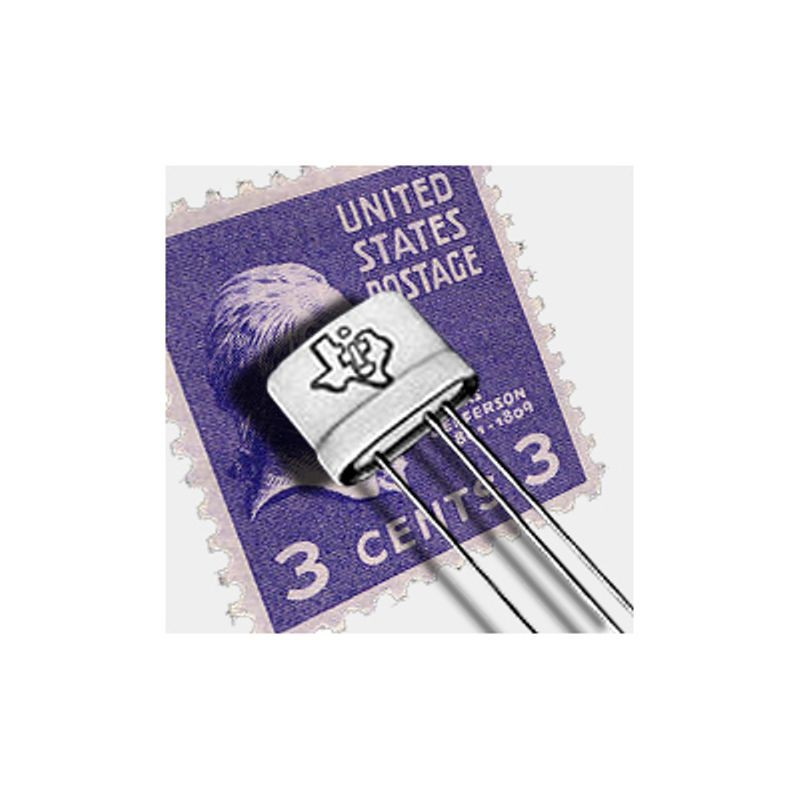
\includegraphics[scale = 0.2]{Graphics/texas_instruments_silicon_transistor.jpg}
	\caption{\textbf{Transistor} de \textbf{silicio} de \emph{Texas Instruments}, anunciando su pequeño tamaño.}
	\label{fig:5}
\end{figure}

Ambos dispositivos se fabricaron controlando el dopaje de cristales de \textbf{silicio} individuales mientras crecían a partir de \textbf{silicio} fundido. \emph{Morris
Tanenbaum} y \emph{Calvin S. Fuller} desarrollaron un método superior en los \emph {Laboratorios Bell} a principios de 1955 mediante la difusión gaseosa de impurezas
donantes y aceptadoras en chips de \textbf{silicio} monocristalinos.\\
Sin embargo, hasta finales de la década de 1950, el \textbf{germanio} siguió siendo el material semiconductor dominante para los transistores y otros dispositivos
semiconductores. El \textbf{germanio} se consideró inicialmente el material semiconductor más eficaz, ya que podía demostrar un mejor rendimiento debido a una mayor
movilidad de los portadores. La relativa falta de rendimiento en los primeros semiconductores de \textbf{silicio} se debió a que la conductividad eléctrica estaba
limitada por estados superficiales cuánticos inestables, que impedían que la electricidad penetrara de manera confiable en la superficie para llegar a la capa de \textbf
{silicio} semiconductor.\\

\begin{figure}[htb]
	\centering
	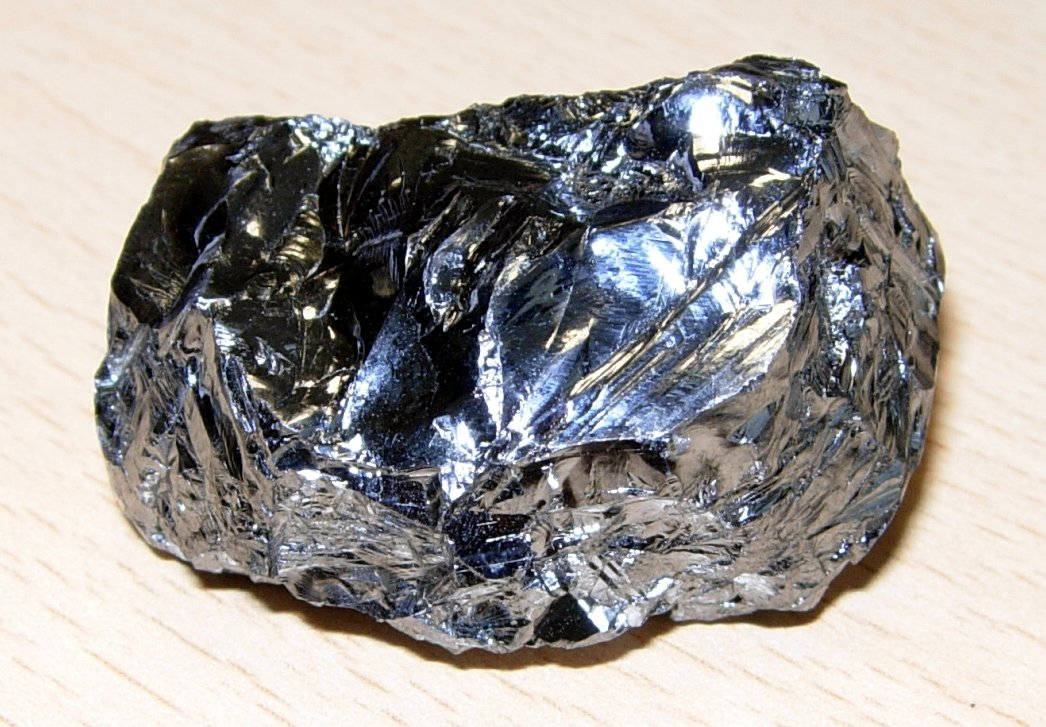
\includegraphics[scale = 0.2]{Graphics/silicon.jpg}
	\caption{Mineral de silicio}
	\label{fig:6}
\end{figure}

En 1955, \emph{Carl Frosch} y \emph{Lincoln Derick} de \emph{Bell Telephone Laboratories}(\textbf{BTL}) descubrieron accidentalmente que el dióxido de \textbf{silicio}(SiO2)
podía crecer sobre \textbf{silicio}. Demostraron que la capa de óxido evitaba que ciertos dopantes entraran en la oblea de \textbf{silicio}, mientras que permitía otros,
descubriendo así el \textbf{efecto pasivante} de la oxidación en la superficie del semiconductor. En la década de 1950, \emph{Mohamed Atalla}, retomó el trabajo de \emph{Frosch}
sobre la oxidación, investigó las propiedades superficiales de los semiconductores de \textbf{silicio} en los \emph{Laboratorios Bell}, donde propuso un nuevo método de fabricación
de dispositivos semiconductores, recubriendo una oblea de \textbf{silicio} con una capa aislante de óxido de \textbf{silicio} para que la electricidad podría penetrar de manera
confiable en el \textbf{silicio} conductor que se encuentra debajo, superando los estados superficiales que impedían que la electricidad llegara a la capa semiconductora. Esto
se conoce como \textbf{pasivación superficial}, un método que se volvió fundamental para la industria de los semiconductores, ya que más tarde hizo posible la producción en masa de
circuitos integrados de \textbf{silicio}.

\chapter{El microchip}\label{chapter:microchip}



\chapter{El microprocesador}\label{chapter:microprocesador}


El microprocesador es un procesador de computadora, donde la lógica del procesamiento de datos y el control
están incluidos en un solo circuito integrado, o en un pequeño número de circuitos integrados.
El microprocesador contiene los circuitos aritméticos, lógicos y de control necesarios para realizar 
las funciones de la unidad central de procesamiento  de una computadora. El circuito integrado es capaz de interpretar y 
ejecutar instrucciones de programa y realizar operaciones aritméticas. 
El microprocesador es un circuito integrado digital multipropósito, controlado por reloj y basado en registros que 
acepta datos binarios como entrada, los procesa de acuerdo con las instrucciones almacenadas en su memoria y proporciona 
resultados (también en forma binaria) como salida. Un microprocesador hipotético minimamente funcional podría incluir
solo una \textbf{ALU}(\emph{aritmetic logic unit }) y una sección lógica de control. La \textbf{ALU} realiza sumas, restas 
y operaciones como \textbf{AND} y \textbf{OR}. Cada operación de la \textbf{ALU} establece uno o más \emph{flags} en un registro 
de estados, que indican los resultados de la última operación(por ejemplo, si el resultado es cero, si es negativo, si 
hay desbordamiento, etc.). La lógica de control recupera los código de instrucción desde la memoria e inicia la secuencia de
operaciones necesarias parar que la \textbf{ALU} lleve a cabo la instrucción\brackcite{wikipedia_2022_Microprocesador}.
\\ Antes de los microprocesadores las computadoras pequeñas se construían utilizando  \emph{racks} de placas de circuito con 
muchos circuitos integrados de mediana y pequeña escala, generalmente del tipo \textbf{TTL}\emph{(Transistor-Transistor Logic)} 
\brackcite{wikipedia_2022_ttl}. Los microprocesadores combinaron esto en uno o unos pocos circuitos integrados a gran escala.\\
El incremento continuo de las capacidades de los microprocesadores desde  que 
se empezaron a fabricar ha dejado otras formas de computadoras casi complemtamente
obsoletas, con uno o más microprocesadores usados en todo desde pequeños sistemas 
embebidos  y dispostivos portátiles hasta los enormes \emph{mainframes} y las supercomputadoras

\section{Surgimiento del microprocesadaor}
Las invenciones a veces ocurren cuando las personas se enfrentan a un problema y luchan por resolverlo. En otras ocasiones, suceden 
cuando las personas adoptan una meta visionaria. La historia de cómo Ted Hoff y su equipo de Intel inventaron el microprocesador es 
un caso de ambos \brackcite{isaacson_2014}. Hoff, que había sido un joven profesor en Stanford, se convirtió en el duodécimo empleado 
de Intel, donde fue asignado para trabajar en el diseño de chips. Hoff se dio cuenta de que era un desperdicio y poco elegante diseñar 
muchos tipos de microchips donde cada uno tuviera una función diferente,  que era lo que \textbf{Intel} estaba haciendo hasta ahora. 
Llegaría una empresa y le pediría que construyera un microchip diseñado para realizar una tarea específica. Hoff imaginó, al igual que 
Noyce y otros, un enfoque alternativo: crear un chip de propósito general que pudiera ser instruido o programado para realizar una 
variedad de aplicaciones diferentes según se desee. En otras palabras, una computadora de propósito general en un chip. 
Esta visión coincidió con un problema que se planteó a Hoff en el verano de 1969. Una empresa japonesa llamada Busicom 
estaba planeando una nueva y poderosa calculadora de escritorio : la \textbf{Busicom 141-PF}, y había elaborado especificaciones para doce microchips de propósito especial 
para diseñar 12 chips personalizados para su nueva calculadora de impresión (diferentes para manejar pantalla, cálculos, memoria, etc.) que quería que Intel construyera. 
Intel estuvo de acuerdo y se fijó un precio. Noyce le pidió a Hoff que supervisara el proyecto. La cantidad de chips y su 
complejidad fue mucho mayor de lo que esperaba, por lo que no había forma de que \textbf{Intel} pudidiera construirlos al precio acordado.
Hoff propuso que Intel diseñara un solo chip lógico que pudiera realizar casi todas las tareas que quería Busicom.
Para empeorar las cosas,  la creciente popularidad de la calculadora de bolsillo de Jack Kilby estaba obligando a Busicom a reducir aún más su precio.
.Noyce le dijo a Hoff que lo intentara y  tuvo que convencer a Grove del proyecto antes de venderle la idea a Busicom. En septiembre de 1969, Hoff y 
su colega Stan Mazor habían esbozado la arquitectura de un chip lógico de uso general que podía seguir instrucciones de programación. 
Sería capaz de hacer el trabajo de nueve de los doce chips que había solicitado Busicom.
Se diseñaron un conjunto cuatro chips conocido como MCS-4. Incluía un chip de unidad de procesamiento central (CPU), el 4004, así como un chip de memoria 
de solo lectura (ROM) compatible para los programas de aplicaciones personalizadas, un chip de memoria de acceso aleatorio (RAM) para procesar datos, y un 
chip de registro para el puerto de entrada/salida (E/S). Cuando llegó el momento de renegociar el precio, Hoff hizo una recomendación fundamental a Noyce, 
que ayudó a crear un gran mercado para los chips de uso general y aseguró que Intel seguiría siendo un impulsor de la era digital.
A cambio de darle a Busicom un buen precio, Noyce insistió en que Intel retuviera los derechos del nuevo chip y se le permitiera licenciarlo a otras 
compañías para fines distintos a la fabricación de una calculadora. Debido a que era esencialmente un procesador de computadora en un chip, el nuevo dispositivo 
se denominó microprocesador. En noviembre de 1971 Intel dio a conocer el producto, el Intel 4004, al público. Este tenía un precio de salida de \$ 200
\brackcite{intel_4004,wikipedia_2022_Microprocesador,campbell-kelly_garcia-swartz_2015,isaacson_2014}.

\begin{figure}[htb]
	\centering
	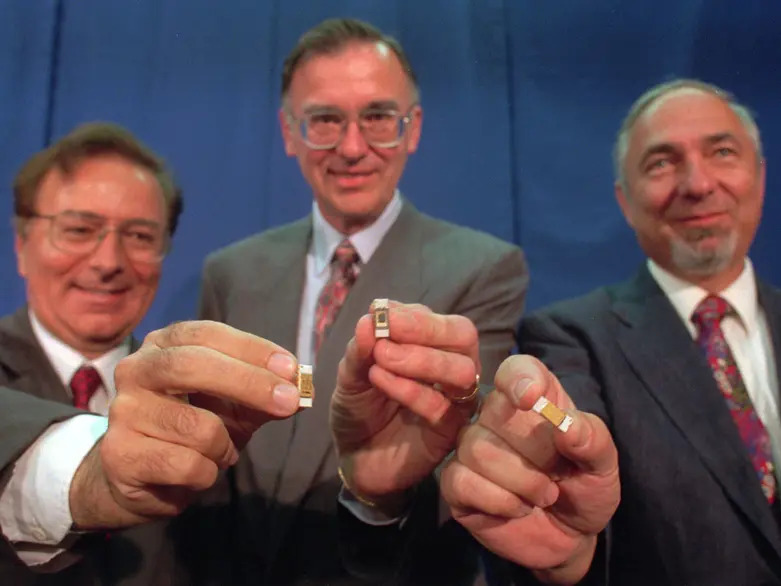
\includegraphics[scale = 0.25]{Graphics/faggin_hoff_mazor_-4004.jpg}
	\caption{Desde la isquierda, Federico Faggin, Ted Hoff y Stanley Mazor con procesadores Intel 4004}
	\label{fig:10}
\end{figure}

\subsection{Intel 4004}

Este revolucionario \textbf{microprocesador}, del tamaño de la uña del dedo meñique, entregaba la misma potencia de cómputo que la primera computadora electrónica construida 
en 1946, que llenó una habitación entera. El primer microprocesador Intel 4004 se fabricó en obleas de dos pulgadas, en comparación con las obleas de 12 
pulgadas que se utilizan habitualmente en los productos actuales. El microprocesador Intel 4004 es único en el sentido de que es uno de los diseños de 
microprocesador más pequeños que alguna vez entró en producción comercial. El 4004  era un microprocesador de \textbf{4-bits}, alcanzaba 
una máxima velocida de reloj 740 kHz. El ancho de línea del circuito del microprocesador Intel 4004 era de 10 micrones o 10 000 nanómetros. 
En 1971 el Intel 4004 contenía 2300 transistores Para el 2010, un procesador Intel Core con matriz de procesamiento de 32 nm y tecnología de silicio de puerta metálica de alta k de 
segunda generación contenía  560 millones de transistores. En comparación, un cabello humano promedio tiene 100,000 nanómetros de ancho \brackcite{intel_4004,wikipedia_2022_intel_4004}.      

\begin{figure}[htb]
	\centering
	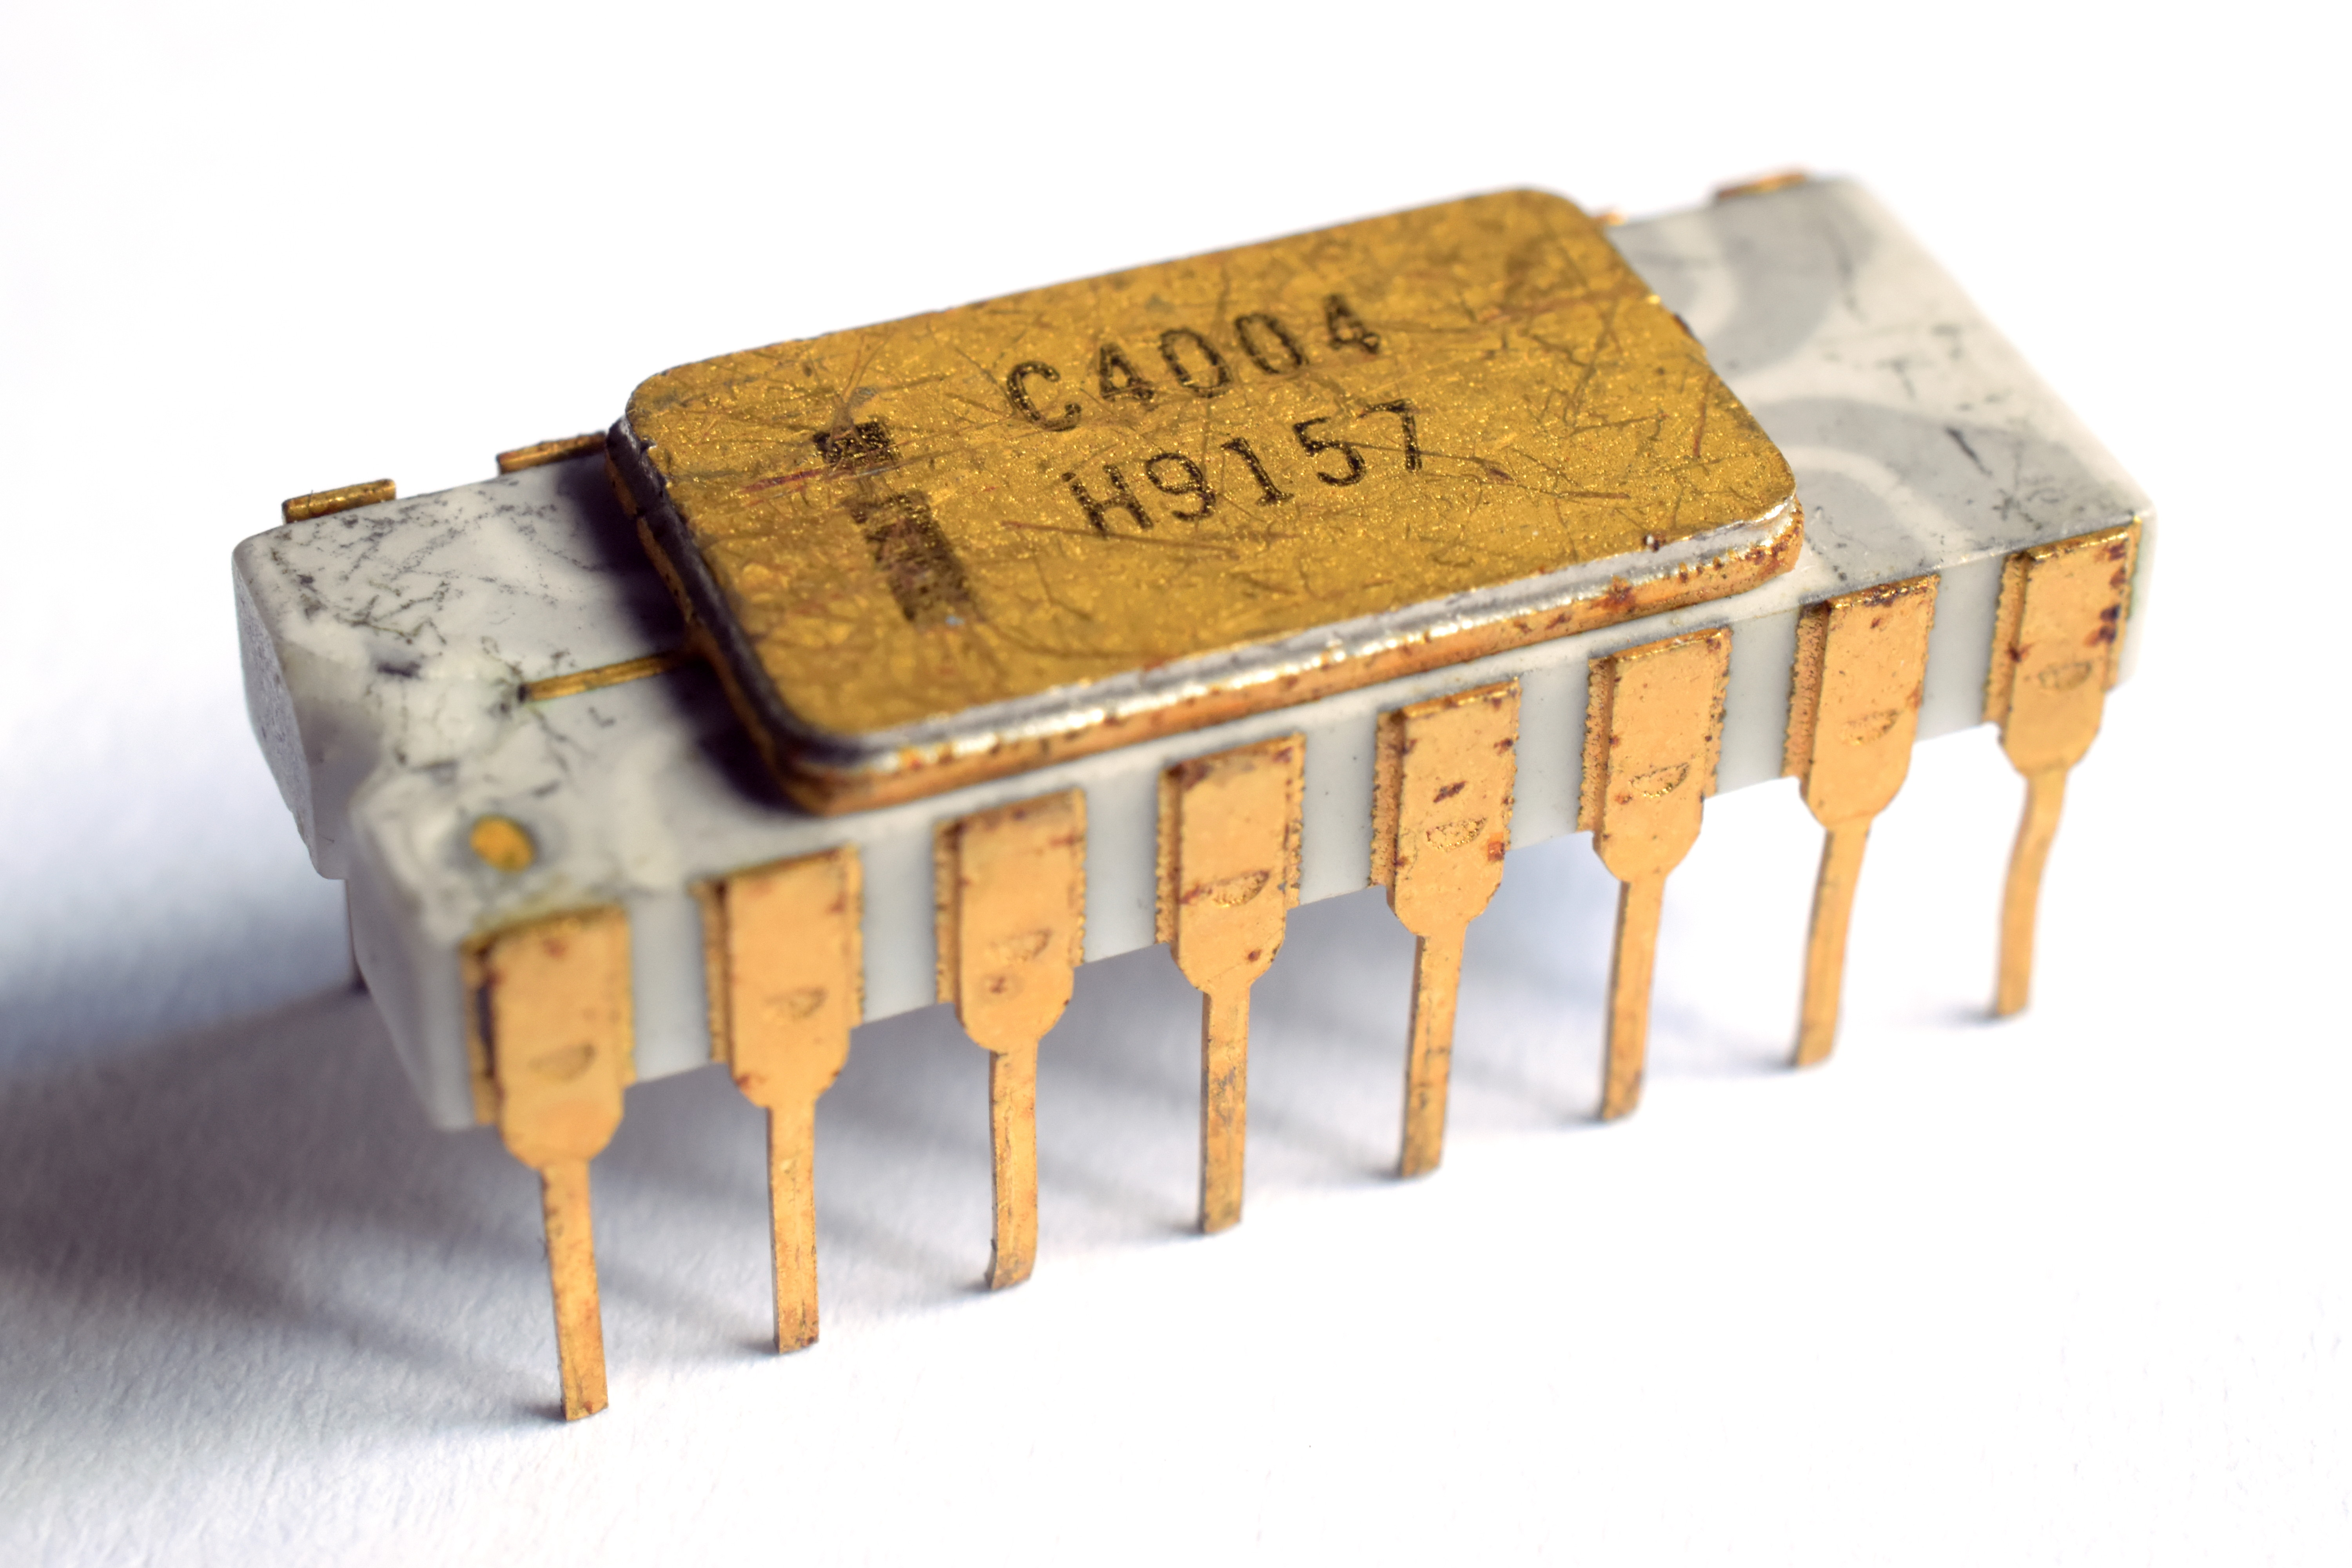
\includegraphics[scale = 0.15]{Graphics/Intel_C4004.jpg}
	\caption{Primer microprocesador :\textbf{Intel 4004}}
	\label{fig:12}
\end{figure}


\section{El arribo del primer microprocesador de 8 bits}

El Intel 4004 fue seguido en 1972 por el Intel 8008, el primer microprocesador de 8 bits del mundo. Sin embargo, el 8008 no fue una extensión del diseño del 4004, 
sino la culminación de un proyecto de diseño separado en Intel, que surgió de un contrato con Computer Terminals Corporation, por un chip para una 
terminal que estaban diseñando, el Datapoint 2200: los aspectos fundamentales del diseño no provinieron de Intel sino de CTC. 
El 8008 salió con 3.500 transistores, tenía un bus de datos de 8 bits y un bus de direcciones de 14 bits. Este micoprocesaddor fue la base del famoso kit de 
computadora "Mark-8" \brackcite{wikipedia_2022_intel_8008,campbell-kelly_garcia-swartz_2015}.
\begin{figure}[htb]
	\centering
	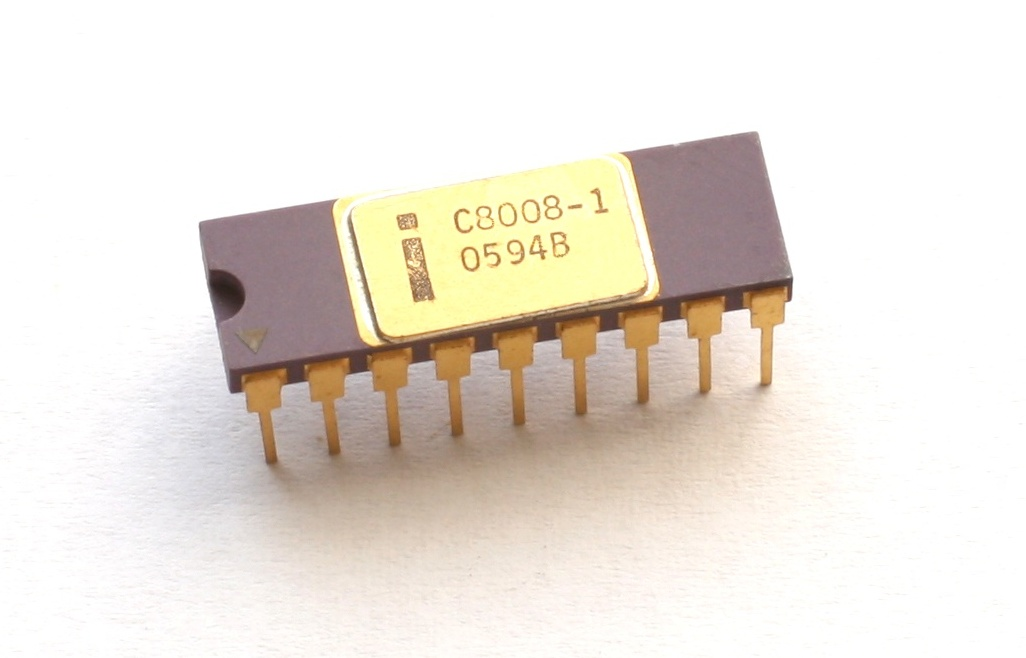
\includegraphics[scale = 0.15]{Graphics/Intel_C8008-1.jpg}
	\caption{Microprocesador  \textbf{Intel 8008}}
	\label{fig:13}
\end{figure}

\subsection{8080}
El Intel 8080 es el segundo microprocesador de 8 bits diseñado y fabricado por Intel. Apareció por primera vez en abril de 1974 y es una variante ampliada y mejorada
del diseño anterior del 8008, aunque sin compatibilidad binaria. La velocidad de reloj o límite de frecuencia especificado inicialmente era de 2 MHz, con instrucciones
comunes que usaban 4, 5, 7, 10 o 11 ciclos. Como resultado, el procesador podía ejecutar varios cientos de miles de instrucciones por segundo. Federico Faggin lo concibió 
y diseñó utilizando MOS de canal N de alto voltaje.

\begin{figure}[htb]
	\centering
	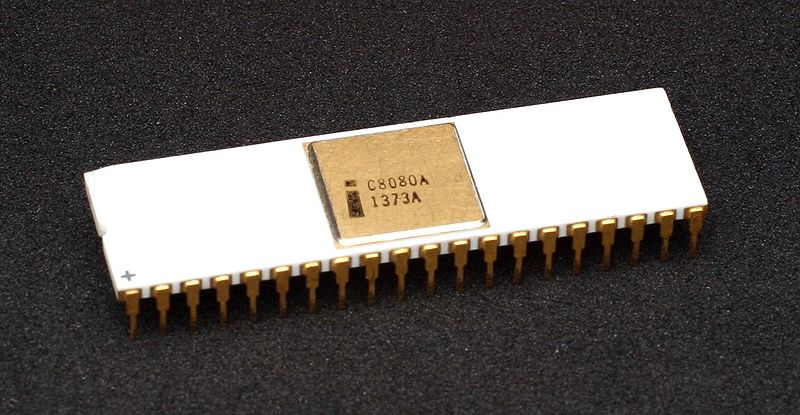
\includegraphics[scale = 0.2]{Graphics/8080_microprocessorr.jpg}
	\caption{Microprocesador  \textbf{Intel 8080}}
	\label{fig:14}
\end{figure}

\section{El arribo de los 16 bits}

El primer microprocesador multichip de 16 bits fue el National Semiconductor IMP-16, presentado a principios de 1973. Una versión de 8 bits del conjunto de 
chips se introdujo en 1974 como IMP-8. Durante el mismo año, National presentó el primer microprocesador de un solo chip de 16 bits, el PACE, seguido de una 
versión NMOS, el INS8900. El primer microprocesador de 16 bits de un solo chip fue el TMS 9900 de TI, presentado en 1976, que también era compatible con su 
línea de minicomputadoras TI-990. Intel produjo su primer procesador de 16 bits, el 8086, en 1978. Era compatible con el 8080 y el 8085 (un derivado del 8080)
\brackcite{wikipedia_2022_Microprocesador,staff_2021_microprocessor}.
\begin{figure}[htb]
	\centering
	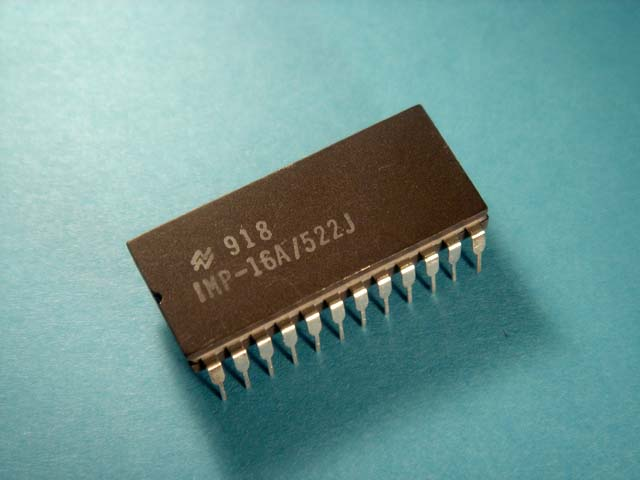
\includegraphics[scale = 0.2]{Graphics/NSIMP-16A.jpg}
	\caption{Microprocesador  IMP-16}
	\label{fig:15}
\end{figure}

\section{8086: El comienzo de x86}
El primer procesador de 16 bits de Intel fue el 8086, que ayudó a mejorar considerablemente el rendimiento en comparación con los diseños anteriores.
Este microprocesador utilizaba la misma microarquitectura que los microprocesadores de 8 bits de Intel (8008, 8080 y 8085). Esto permitió que los programas 
en lenguaje ensamblador escritos en 8 bits migraran sin problemas. El 8086 no solo tenía una frecuencia más alta que la 8088, sino que también empleaba un 
bus de datos externo de 16 bits y una cola de precarga de 6 bytes más larga. También podía ejecutar tareas de 16 bits (aunque la mayoría del software en ese 
momento estaba diseñado para procesadores de 8 bits). El bus de direcciones se amplió a 20 bits, lo que permitió al 8086 acceder a hasta 1 MB de memoria y, 
por lo tanto, aumentar el rendimiento. El 8086 también se convirtió en el primer procesador x86 y utilizó la primera revisión del x86 ISA\brackcite{wikipedia_2022_x86_ISA}, en el que se han 
basado casi todos los procesadores creados por AMD o Intel desde la introducción del 8086 \brackcite{wikipedia_2022_Microprocesador,sexton_2018_history_intel_cpus,wikipedia_2022_intel_8086}.
\begin{figure}[htb]
	\centering
	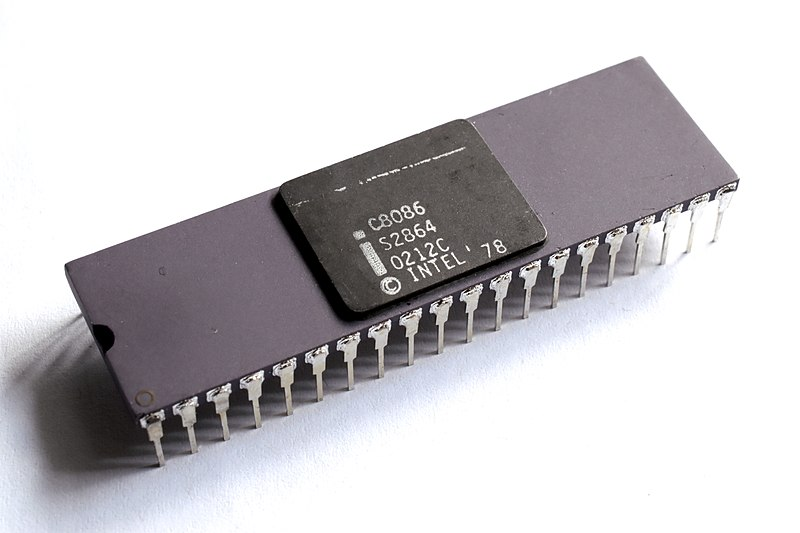
\includegraphics[scale = 0.2]{Graphics/Intel_C8086.jpg}
	\caption{Intel 8086}
	\label{fig:16}
\end{figure}

\section{El arribo de los 32 bits}

% En 1968, Vic Poor y Harry Pyle de CTC 
% desarrollaron el diseño original para el conjunto de instrucciones y el funcionamiento del procesador. En 1969, CTC contrató a dos empresas, Intel y Texas Instruments, para 
% realizar una implementación de un solo chip, conocida como CTC 1201. A fines de 1970 o principios de 1971, TI se retiró al no poder fabricar una pieza confiable. 
% En 1970, con Intel aún por entregar la parte, CTC optó por usar su propia implementación en el Datapoint 2200, usando en su lugar la lógica TTL tradicional 
% (por lo tanto, la primera máquina que ejecutó el "código 8008" no era de hecho un microprocesador y se entregó el año anterior). La versión de Intel del microprocesador 
% 1201 llegó a fines de 1971, pero fue demasiado tarde, lenta y requirió una cantidad de chips de soporte adicionales. CTC no tenía interés en usarlo. CTC había contratado
% originalmente a Intel por el chip y les habría debido 50 000 dólares estadounidenses (equivalente a 334 552 dólares en 2021) por su trabajo de diseño.[43] 
% Para evitar pagar por un chip que no querían (y no podían usar), CTC liberó a Intel de su contrato y les permitió el uso gratuito del diseño.[43] Intel 
% lo comercializó como 8008 en abril de 1972, como el primer microprocesador de 8 bits del mundo. Fue la base del famoso kit de computadora "Mark-8". 

% En 1973, Intel lanzó el primer procesador de 8 bits ampliamente utilizado, llamado Intel 8008. El 8008 salió con 3.500 transistores. . En este sistema, el bus de datos y 
% las direcciones eran unidades de 8 bits. El Intel 4004 fue seguido en 1972 por el Intel 8008, el primer microprocesador de 8 bits del mundo. Sin embargo, el 8008 no fue 
% una extensión del diseño del 4004, sino la culminación de un proyecto de diseño separado en Intel, que surgió de un contrato con Computer Terminals Corporation, de San Antonio TX, 
% por un chip para una terminal que estaban diseñando, [42] el Datapoint 2200: los aspectos fundamentales del diseño no provinieron de Intel sino de CTC.



 % Pronto surgió un desafío. “Cuanto más aprendía sobre este diseño, más me 
% preocupaba que Intel pudiera haber emprendido más de lo que estaba preparado para entregar”, recordó Hoff. "La cantidad de chips y su 
% complejidad fue mucho mayor de lo que esperaba". No había forma de que Intel pudiera construirlos al precio acordado. .
% Hoff propuso que Intel diseñara un solo chip lógico que pudiera realizar casi todas las tareas que quería Busicom

% “Bueno, si hay algo que se te ocurra para simplificar el diseño, ¿por qué no lo persigues?”, sugirió Noyce.
% . 
% “Sé que esto se puede hacer”, dijo sobre el chip de propósito general. “Se puede hacer para emular una computadora”. 
% Noyce le dijo que lo intentara. 
% Antes de que pudieran vender la idea a Busicom, Noyce se dio cuenta de que tenía que convencer a alguien que podría oponerse 
% aún más: Andy Grove, quien nominalmente trabajaba para él. Parte de lo que Grove vio como su mandato era mantener a Intel enfocado.

% Noyce diría que sí a casi cualquier cosa; El trabajo de Grove era decir que no. Cuando Noyce se acercó al espacio de trabajo de Grove y se 
% sentó en la esquina de su escritorio, Grove se puso inmediatamente en guardia. Sabía que el esfuerzo de Noyce por parecer indiferente era una 
% señal de que algo estaba pasando. “Estamos comenzando otro proyecto”, dijo Noyce, fingiendo reír.53 La primera reacción de Grove fue decirle a 
% Noyce que estaba loco. Intel era una empresa incipiente que todavía luchaba por fabricar sus chips de memoria y no necesitaba distracciones. Pero 
% después de escuchar a Noyce describir la idea de Hoff, Grove se dio cuenta de que la resistencia probablemente estaba mal y definitivamente era inútil.
% En septiembre de 1969, Hoff y su colega Stan Mazor habían esbozado la arquitectura de un chip lógico de uso general que podía seguir instrucciones de programación. 
%  Noyce y Hoff presentaron la opción a los ejecutivos de Busicom, 
% quienes acordaron que era el mejor enfoque.

% .  Fue un punto de negociación que Bill Gates y Microsoft emularían con IBM una década después. 
% A cambio de darle a Busicom un buen precio, Noyce insistió en que Intel retuviera los derechos del nuevo chip y se le permitiera licenciarlo a otras compañías 
% para fines distintos a la fabricación de una calculadora. 

% Se dio cuenta de que un chip que pudiera programarse para realizar cualquier función lógica se convertiría en un componente estándar en los dispositivos electrónicos, 
% de la misma manera que las piezas de madera de dos por cuatro eran un componente estándar en la construcción de casas.
% Reemplazaría los chips personalizados, lo que significaba que podría fabricarse a granel y, por lo tanto, su precio disminuiría continuamente. También marcaría el 
% comienzo de un cambio más sutil en la industria electrónica: la importancia de los ingenieros de hardware, que diseñaron la 

% ubicación de los componentes en una placa de circuito, comenzó a ser suplantada por una nueva generación, los ingenieros de software, cuyo trabajo era programar 
% Debido a que era esencialmente un procesador de computadora en un chip, el nuevo dispositivo se denominó microprocesador. En noviembre de 1971 Intel dio a conocer 
% el producto, el Intel 4004, al público. Sacó anuncios en revistas especializadas que anunciaban “una nueva era de electrónica integrada: ¡una computadora microprogramable en 
% un chip!” Tenía un precio de \$ 200 y los pedidos, así como miles de solicitudes del manual, comenzaron a llegar. Noyce asistía a una exhibición de computadoras en 
% Las Vegas el día del anuncio y estaba emocionado de ver a los clientes potenciales abarrotar la suite de Intel.

% 1969: La misión
% En 1969, Nippon Calculating Machine Corporation se acercó a Intel para diseñar 12 chips personalizados para su nueva calculadora de impresión Busicom 141-PF*. 
% Los ingenieros de Intel sugirieron una familia de solo cuatro chips, incluido uno que podría programarse para su uso en una variedad de productos, poniendo en 
% marcha una hazaña de ingeniería que alteró drásticamente el curso de la electrónica.


% 1971: era de la electrónica integrada
% Intel compró los derechos de Nippon Calculating Machine Corporation y lanzó el procesador Intel® 4004 y su conjunto de chips con un anuncio en la edición del 15 de noviembre 
% de 1971 de Electronic News: "Anunciando una nueva era en la electrónica integrada".
% Fue entonces cuando Intel® 4004 se convirtió en el primer procesador programable de uso general del mercado: un "bloque de construcción" que los ingenieros podían comprar y 
% luego personalizar con software para realizar diferentes funciones en una amplia variedad de dispositivos electrónicos.

% oderosamente pequeño, incluso en 1971
% Este microprocesador revolucionario, del tamaño de la uña del dedo meñique, entregaba la misma potencia de cómputo que la primera computadora electrónica construida en 
% 1946, que llenó una habitación entera.





\backmatter

% \include{BackMatter/Conclusions}
% \include{BackMatter/Recomendations}
\printbibliography[heading=bibintoc]




\end{document}
